\documentclass[a4paper, 11pt, titlepage]{article}

\usepackage{setspace}
\onehalfspacing

\usepackage[utf8]{inputenc}
\usepackage[T1]{fontenc}
\usepackage[english]{babel}

\usepackage{color}
\usepackage{float}
\usepackage{fancyvrb}

\usepackage{amssymb}
\usepackage{amsmath}
\usepackage{listings}
\usepackage{comment} 

\usepackage{caption}
\usepackage{subcaption}

\usepackage{graphicx}
\DeclareGraphicsExtensions{.jpg}

\usepackage{enumitem}
\setlist[description]{itemsep=-2mm, topsep=0mm, itemindent=-4mm}

\definecolor{dkgreen}{rgb}{0,0.45,0}
\definecolor{gray}{rgb}{0.5,0.5,0.5}
\definecolor{mauve}{rgb}{0.30,0,0.30}

\lstset{frame=tb,
  language=Python,
  aboveskip=4mm,
  belowskip=5mm,
  showstringspaces=false,
  columns=flexible,
  basicstyle={\small\ttfamily},
  numbers=left,
  numberstyle=\footnotesize,
  keywordstyle=\color{dkgreen}\bfseries,
  commentstyle=\color{dkgreen},
  stringstyle=\color{mauve},
  frame=single,
  breaklines=true,
  breakatwhitespace=false,
  tabsize=4,
}

\captionsetup[figure]{aboveskip=0mm}
\captionsetup[subfigure]{aboveskip=0mm}

\usepackage{dirtytalk}

\usepackage[hidelinks]{hyperref}

\usepackage{pgfplots}
\pgfplotsset{
    box plot/.style={
        /pgfplots/.cd,
        black,
        only marks,
        mark=-,
        mark size=1em,
        /pgfplots/error bars/.cd,
        y dir=plus,
        y explicit,
    },
    box plot box/.style={
        /pgfplots/error bars/draw error bar/.code 2 args={%
            \draw  ##1 -- ++(1em,0pt) |- ##2 -- ++(-1em,0pt) |- ##1 -- cycle;
        },
        /pgfplots/table/.cd,
        y index=2,
        y error expr={\thisrowno{3}-\thisrowno{2}},
        /pgfplots/box plot
    },
    box plot top whisker/.style={
        /pgfplots/error bars/draw error bar/.code 2 args={%
            \pgfkeysgetvalue{/pgfplots/error bars/error mark}%
            {\pgfplotserrorbarsmark}%
            \pgfkeysgetvalue{/pgfplots/error bars/error mark options}%
            {\pgfplotserrorbarsmarkopts}%
            \path ##1 -- ##2;
        },
        /pgfplots/table/.cd,
        y index=4,
        y error expr={\thisrowno{2}-\thisrowno{4}},
        /pgfplots/box plot
    },
    box plot bottom whisker/.style={
        /pgfplots/error bars/draw error bar/.code 2 args={%
            \pgfkeysgetvalue{/pgfplots/error bars/error mark}%
            {\pgfplotserrorbarsmark}%
            \pgfkeysgetvalue{/pgfplots/error bars/error mark options}%
            {\pgfplotserrorbarsmarkopts}%
            \path ##1 -- ##2;
        },
        /pgfplots/table/.cd,
        y index=5,
        y error expr={\thisrowno{3}-\thisrowno{5}},
        /pgfplots/box plot
    },
    box plot median/.style={
        /pgfplots/box plot
    }
}

\begin{comment}
\begin{lstlisting}[language=python]
her kan i vise kode som i forklarer.
indryk virker fint her.
\end{lstlisting}
\end{comment}

\title{First year project\\Project 99: Who's Julia?\\\rule{10cm}{0.5mm}}
\author{Group: 99a - Supervisor: Michal Kotrbcik\\Simon Lehmann Knudsen, simkn15\\Sonni Hedelund Jensen, sonje15\\Asbjørn Mansa Jensen, asjen15
	\\ FF501\\\rule{5.5cm}{0.5mm}\\}
\date{\today}

%Pagestyling
\usepackage{lastpage}
\usepackage{fancyhdr}
\pagestyle{fancy}
\fancyhf{}
\lhead{simkn15, sonje15, asjen15}
\rhead{Project 99: Who's Julia?}
\cfoot{\thepage}

\begin{document}

\maketitle

\vfill

\newpage
\pagenumbering{roman}
\section{Summary}
Julia is a new programming language. Through tests and benchmarking it is found that Julia does some optimizations behind the scene but these optimizations does not seem as developed as Javas optimizations. In most of the tests in this report and the Project Euler solutions that was not included in the report showed that Julia is relatively fast even in this early stage of development. This is what the developers state and with what seems like a lot of inspiration from Python, they managed to create an easy to learn and easy to write programming language.

\newpage
\tableofcontents

\newpage
\pagenumbering{arabic}
\pagestyle{fancy}
\fancyhf{}
\lhead{simkn15, sonje15, asjen15}
\rhead{Project 99: Who's Julia?}
\cfoot{\thepage\ of \pageref{LastPage}}
\section{Introduction}
Java, C++ and Python are on the top ten of the most used programming languages. There are hundreds of languages, but not minding the hard competition, new languages are still created with the thought of doing better. An example of this is the relatively new programming language Julia, which has been developed with the idea to combine the best features of other languages.\\
\\
The purpose of this report is to find out how well Julia perform compared to some of the standard languages as of 2016. One of those languages is Python which Julia draws a lot of inspiration from, including syntax and the dynamic type system. The second language that Julia will be compared with is Java, these two do share similarities, but most of the similarities are behind the scene mechanics, such as garbage collection and compiler optimizations. The developers of Julia claim that Julia is as fast as C. Therefore we choose C++ as the last language to compare Julia with.
\\
The report starts introducing Julia, Julia's background and features. Julia's introduction is followed by a brief introduction to Project Euler. Next we outline our approach to benchmarking, profiling, and time measurements used in the experimental part of the project. Next op is the materials and methods used for benchmarking followed by the problems/algorithms used for benchmarking. The results, personal experiences learning Julia, discussion and conclusion will come at last. 

\section{Julia}
In this section we introduce Julia and compare its syntax with the syntax of Python, C++ and Java. Julia's homepage lists the follwing as the core and crucial features of the language:
\begin{description}
	\item[$\cdot$] Dynamic typing and byte-related memory management
	\item[$\cdot$] Multiple dispatch
	\item[$\cdot$] User defined types
	\item[$\cdot$] Garbage Collector
	\item[$\cdot$] Built-in package manager
	\item[$\cdot$] Lightweight green threading
	\item[$\cdot$] Meta-programming and Macros
	\item[$\cdot$] Automatic generation of efficient, specialized code for different argument types
	\item[$\cdot$] Implementing code from other languages
	\item[$\cdot$] Designed for parallelism and distributed computation
	\item[$\cdot$] Supports Unicode
	\item[$\cdot$] Elegant and extensible conversions and promotions for numeric and other types
	\item[$\cdot$] Devectorized code is fast
	\item[$\cdot$] Others we have not looked in to
\end{description}
We will later conclude this by a brief explanation of some of these features and concepts.\\
\\
Julia is an object-oriented programming language, which has been under development since 2009. First released in 2012 and the newest stable version of Julia is version 0.4.5. The language has been created because the developers wanted a language with all the features they like from other languages. The developers wanted the language to be open source, which means that everybody can read and modify the language. One of the ideas was to make the language as simple, readable and easy to learn as possible. The language is made for high performance and scientific computations while still supporting general purpose programming. 
Programming in Julia can be done in the terminal like Python with interactive mode:
\begin{figure}[H]
	\centering
	\begin{subfigure}[H]{0.8\textwidth}
		\centering
		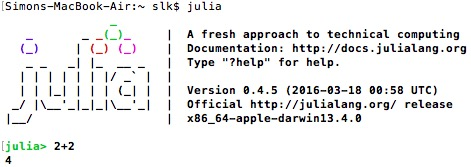
\includegraphics
		[width=\textwidth]{image/terminalj.jpg} 
		\caption{Julia}.
	\end{subfigure}	
	\begin{subfigure}[H]{0.8\textwidth}
		\centering
		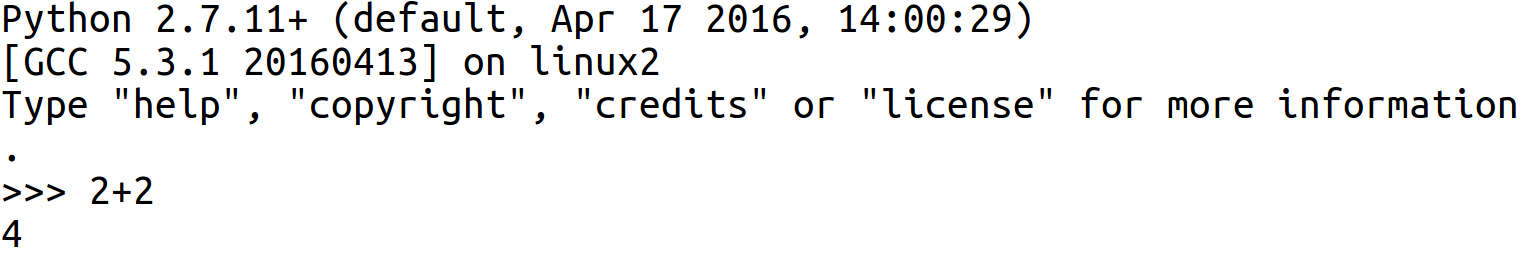
\includegraphics
		[width=\textwidth]{image/terminalp.jpg} 
		\caption{Python}.
	\end{subfigure}
	\caption{Julia and Python in terminal}
\end{figure}

Writing longer programs in the terminal might not be the preferred method. Files containing Julia code can be interpreted by the Julia's interpreter with the following command from terminal:\\
\textbf{julia test.jl}\\
The text editor Atom supports the Julia language. Atom has a package, \textbf{uber-juno}, which sets up Atom to act like an IDE, integrated development environment for Julia. However, the programmer can of course use whatever text editor he or she likes.

\subsection{Syntax}
\begin{figure}[H]
	\begin{lstlisting}[language=python]
	Julia:	    Python:      Java:            c++:
	a = 10	    a = 10       int a = 10;      int a = 10;
	\end{lstlisting}
	\caption{Declaring and assigning variables}
	\label{variables}
\end{figure}

\begin{figure}[H]
	\centering
	\begin{subfigure}[H]{0.7\textwidth}
		\centering
		\begin{lstlisting}[belowskip=0.5mm]
		for i = 1 : 10
			println(i)
		end
		\end{lstlisting}
		\caption{Julia}
	\end{subfigure}
	\begin{subfigure}[H]{0.7\textwidth}
		\centering
		\begin{lstlisting}[belowskip=0.5mm]
		for i in range(1, 11):
			print i
		\end{lstlisting}
		\caption{Python}
	\end{subfigure}	
	\begin{subfigure}[H]{0.7\textwidth}
		\centering
		\begin{lstlisting}[belowskip=0.5mm]
		for (int i = 1; i <= 10; i++){
			System.out.println(i);
		}
		\end{lstlisting}
		\caption{Java}
	\end{subfigure}
	\begin{subfigure}[H]{0.7\textwidth}
		\centering
		\begin{lstlisting}[belowskip=0.5mm]
		for (int i = 1; i <= 1+; i++){
			std::cout << i << "\n";
		}
		\end{lstlisting}
		\caption{C++}
	\end{subfigure}
	\caption{For-loops: Incrementing}
	\label{forloop+}
\end{figure}

\begin{figure}[H]
	\centering
	\begin{subfigure}[H]{0.7\textwidth}
		\centering
		\begin{lstlisting}[belowskip=0.5mm]
		for i = 10 : -1 : 1
			println(i)
		end
		\end{lstlisting}
		\caption{Julia}
	\end{subfigure}
	\begin{subfigure}[H]{0.7\textwidth}
		\centering
		\begin{lstlisting}[belowskip=0.5mm]
		for i in range(10, 0, -1):
			print i
		\end{lstlisting}
		\caption{Python}
	\end{subfigure}	
	\begin{subfigure}[H]{0.7\textwidth}
		\centering
		\begin{lstlisting}[belowskip=0.5mm]
		for (int i = 10; i > 0; i--){
			System.out.println(i);
		}
		\end{lstlisting}
		\caption{Java}
	\end{subfigure}
	\begin{subfigure}[H]{0.7\textwidth}
		\centering
		\begin{lstlisting}[belowskip=0.5mm]
		for (int i = 10; i > 0; i--){
			std::cout << i << "\n";
		}
		\end{lstlisting}
		\caption{C++}
	\end{subfigure}
	\caption{For-loops: Decrementing}
	\label{forloop-}
\end{figure}

\begin{figure}[H]
	\centering
	\begin{subfigure}[H]{0.7\textwidth}
		\centering
		\begin{lstlisting}[belowskip=0.5mm]
		if i == a
			println(a * b)
		end
		elseif i == b
			println(a / b)
		else
			println(a + b)
		end
		\end{lstlisting}
		\caption{Julia}
	\end{subfigure}
	\begin{subfigure}[H]{0.7\textwidth}
		\centering
		\begin{lstlisting}[belowskip=0.5mm]
		if i == a:
			print a * b
		elif i == b:
			print a / b
		else:
			print a + b
		\end{lstlisting}
		\caption{Python}
	\end{subfigure}	
	\begin{subfigure}[H]{0.7\textwidth}
		\centering
		\begin{lstlisting}[belowskip=0.5mm]
		if(i == a){
			System.out.println(a * b);
		}
		else if(i == b){
			System.out.println(a / b);
		}
		else{
			System.out.println(a + b);
		}
		\end{lstlisting}
		\caption{Java}
	\end{subfigure}
	\begin{subfigure}[H]{0.7\textwidth}
		\centering
		\begin{lstlisting}[belowskip=0.5mm]
		if(i == a){
			std::cout << a * b << "\n";
		}
		else if(i == b){
			std::cout << a / b << "\n";
		}
		else{
			std::cout << a + b << "\n";
		}
		\end{lstlisting}
		\caption{C++}
	\end{subfigure}
	\caption{If statements}
	\label{ifelse}
\end{figure}

\begin{figure}[H]
	\centering
	\begin{subfigure}[H]{0.7\textwidth}
		\centering
		\begin{lstlisting}[belowskip=0.5mm]
		i = 0
		while i < 10
			i += 1
		end
		\end{lstlisting}
		\caption{Julia}
	\end{subfigure}
	\begin{subfigure}[H]{0.7\textwidth}
		\centering
		\begin{lstlisting}[belowskip=0.5mm]
		i = 0
		while (i < 10):
			i += 1
		\end{lstlisting}
		\caption{Python}
	\end{subfigure}	
	\begin{subfigure}[H]{0.7\textwidth}
		\centering
		\begin{lstlisting}[belowskip=0.5mm]
		int i = 0;
		while (i < 10){
			i++;
		}
		\end{lstlisting}
		\caption{Java}
	\end{subfigure}
	\begin{subfigure}[H]{0.7\textwidth}
		\centering
		\begin{lstlisting}[belowskip=0.5mm]
		int i = 0;
		while (a < 10){
			i++;
		}
		\end{lstlisting}
		\caption{C++}
	\end{subfigure}
	\caption{while-loop}
	\label{whileloop}
\end{figure}

\begin{figure}[H]
	\centering
	\begin{subfigure}[H]{0.7\textwidth}
		\centering
		\begin{lstlisting}[belowskip=0.5mm]
		function hello(name)
			println("Hello $name")
		end
		\end{lstlisting}
		\caption{Julia}
	\end{subfigure}
	\begin{subfigure}[H]{0.7\textwidth}
		\centering
		\begin{lstlisting}[belowskip=0.5mm]
		def hello(name):
			print "Hello", name
		\end{lstlisting}
		\caption{Python}
	\end{subfigure}	
	\begin{subfigure}[H]{0.7\textwidth}
		\centering
		\begin{lstlisting}[belowskip=0.5mm]
		public static void hello(String name){
			System.out.println("Hello " + name);
		}
		\end{lstlisting}
		\caption{Java}
	\end{subfigure}
	\begin{subfigure}[H]{0.7\textwidth}
		\centering
		\begin{lstlisting}[belowskip=0.5mm]
		void hello(std::string name)
		{
			std::cout << "Hello " << name << std::endl;
		}
		\end{lstlisting}
		\caption{C++}
	\end{subfigure}
	\caption{Declaring functions}
	\label{function}
\end{figure}

\begin{figure}[H]
	\centering
	\begin{subfigure}[H]{0.7\textwidth}
		\centering
		\begin{lstlisting}[belowskip=0.5mm]
		array = fill(0, 100)
		\end{lstlisting}
		\caption{Julia}
	\end{subfigure}
	\begin{subfigure}[H]{0.7\textwidth}
		\centering
		\begin{lstlisting}[belowskip=0.5mm]
		array = [0 for col in range(100)]
		\end{lstlisting}
		\caption{Python}
	\end{subfigure}	
	\begin{subfigure}[H]{0.7\textwidth}
		\centering
		\begin{lstlisting}[belowskip=0.5mm]
		int[] array = new int[100];
		Arrays.fill(array, 0);
		\end{lstlisting}
		\caption{Java}
	\end{subfigure}
	\begin{subfigure}[H]{0.7\textwidth}
		\centering
		\begin{lstlisting}[belowskip=0.5mm]
		std::array<int,100> array;
		array.fill(0);
		\end{lstlisting}
		\caption{C++}
	\end{subfigure}
	\caption{Filling array}
	\label{Filling array with 0's}
\end{figure}

\subsection{Features}
In this section we are writing about some of Julia's features.
\subsubsection{Dynamic typing and byte-related memory management}
Dynamic typing is a type management approach where type checks are mostly performed at runtime, as opposed to static typing, where type checks are made at compile time. Dynamic typing allows the programmer to skip the type declaration and let the dynamic type system handle it. In Julia it is possible to specify types, but mostly it is not necessary. 
Julia makes decisions about how much memory to allocate for variables, but the assigned memory size will not change. This means that if a value that exceeds the allocated memory is assigned to the variable after initialization, then a bug will occur. Another point to notice is that the memory size can be decreased and this will be addressed later under the section Garbage Collector. However, there is a range of memory sizes to chose from when initializing a variable. Julia will by default assign 32 bits to an integer or a floating point if no more memory is needed at initialization, but it is possible to manually chose one of the following:
\begin{description}
	\item[$\cdot$] Signed/unsigned integer - 8, 16, 32, 64 and 128 bits – Int8, UInt8, Int16, UInt16, Int32, UInt32, Int64, UInt64, Int128 and UInt128
	\item[$\cdot$] Floating point - 16, 32 and 64 bits – Float16, Float32 and Float64
	\item[$\cdot$] Boolean – 8 bits - Bool
	\item[$\cdot$] Character – 32 bits - Char
\end{description}
To initialize a variable with a given memory size:
\begin{lstlisting}[language=python]
x = Int8(10)
\end{lstlisting}
But if the variable is later assigned a new value, Julia will automatically allocate 32 bits for the variable or more if needed:
\begin{lstlisting}[language=python]
x = Int8(10)
typeof(x) #Int8
x = 4
typeof(x) #Int32
\end{lstlisting}
If no certain memory size is needed but only a specific type, then abstract types can be used. An abstract type is a form of generalization of a concrete type. For example, 16, 32 and 64 bit floating points are of type AbstractFloat. This is especially useful when the programmer do not know how much memory a certain variable may need. Too little memory will result in a bug and too much memory is a waste. 
\subsubsection{Multiple dispatch}
Multiple dispatch is used to determine which function to call by the type of one or more of the parsed argument(s). This is useful when two functions, with the same name, are declared:

\begin{lstlisting}[language=python]
function a(arg1::Int8)
	println("Int")  
end

function a(arg1::Float16)  
	println("Float")  
end    
\end{lstlisting}
If a variable is declared as an \textbf{Int8} and used as argument in function \textbf{a()}, then Julia will print "Int". If the variable is declared as a \textbf{Float16} and used as argument in function \textbf{a()}, Julia will print "Float". It is possible to use abstract types, so \textbf{arg1::Float16} and \textbf{arg1::Int8} could be changed to \textbf{arg1::AbstractFloat} and \textbf{arg1::AbstractInt}, which will make the function 'a' accept any type of floating point and integer.
\subsubsection{User defined types}
User defined types also known as composite types, give the programmer the option to define new types in Julia. A composite type in Julia could look as the following: 
\begin{lstlisting}[language=python]
type person 
	age::Int16 
	name #a variable, which gets the assigned default type ::Any
end    
\end{lstlisting}
If a variable in a composite type is not specified with any type, the default is \textbf{::Any}, which accept any type. To initialize a composite type, think of it like an object. \textbf{Person = person(21, "Carl")}, and the values can be changed with "\textbf{Person.age = 25}".
In the example above, the type \textbf{person} can now be used like any other of the built-in types in Julia.
\begin{lstlisting}[language=python]
function a(arg1::person)
	println(arg1.age)
end
Person = person(21, "Carl")
a(Person) #Will print 21
\end{lstlisting}
As seen in the above example, composite types give the programmer the option to do objected orientated programming and the developers of Julia claim that user defined types are as fast and compact as built-in types. 

\subsubsection{Garbage Collector}
Julia uses a garbage collector to automatically free the memory when needed. There is no guarantee when the garbage collector will run, but it is possible to schedule garbage collection with a function call, \textbf{gc()}, it will be executed at some point. It is not possible to control exactly when to run the garbage collector, but only put it in queue. One thing to keep in mind is that once a variable is defined in Julia, it will always be present until program termination. The garbage collector does not free the memory of unreachable object, but rather reallocates memory for objects when memory size has changed. Therefore, the only way the garbage collector can free the memory is when an object has been reduced in size, for example:

\begin{lstlisting}[language=python]
A = rand(float32, 10000, 10000) 
A = 0
gc() 
\end{lstlisting}
This code will generate a 10.000$\times$10.000 matrix filled with random 32 bit floating points, which consumes approximately 400MB of memory. When the value \textbf{A} is set to 0 the memory allocated will stay the same until the garbage collection is executed, as in the example above, or on program termination. After the execution of the garbage collector \textbf{A} will use memory equal to an integer of 32 bits, \textbf{Int32}.

\subsubsection{Built-in package manager}
Julia comes with a built in package manager, which keeps track of packages that need to be included for the program to run. It is not necessary to state, which packages needs to be included. For example, when the user calls the sort function, \textbf{sort()}, no package include statement or \textbf{math.sort()} is needed – this is done automatically by the package manager.

\subsubsection{Lightweight green threading}
A thread is lightweight when it shares address space with other threads as opposed to heavyweight threads, which have their own address space. If threads share the same address space, the communication between them is faster and much simpler. The communication between heavyweight threads have to go through pipes or sockets. \\
\\
Green threads are threads that are scheduled not by the operating system but rather by the runtime library or the virtual machine. Green threads do not have to rely on the operating system and can be controlled much better – which means the threads are in user space and not kernel space. (See section~\ref{sec:timemeasure} for explanation of time measurement) As of Julia 0.4.5, multithreading is not available, but in the unstable version 0.5.0 an experimental support of multithreading is available. 

\subsubsection{Meta-programming and Macros}
Meta-programming is a way to write programs which is parsed in to another program. In julia meta-programming can be done by defining macros. For example, the \textbf{@time} macro, which was used extensively in the project. The textbf{@time} is a part of the Julia Standard Library. The textbf{@time} macro takes a function as an argument, and starts a timer before the execution of the code and stops the timer after execution. The time passed and memory allocated is printed to the screen.  Meta-programming and macros are known from Lisp, a programming language, and have been used in early AI research. Figure \ref{macro} shows how to make a macro. To use this macro in a program simply write \textbf{@sayhello(Bob)} in the program, and "Hello, Bob" will be printed to the screen.
\begin{figure}[H]
	\begin{lstlisting}[language=python]
	macro sayhello(name)
		return :( println("Hello, ", $name) )
	end
	\end{lstlisting}
	\caption{Making a macro}
	\label{macro}
\end{figure}

\subsubsection{Implementing code from other languages}
Since Julia is a newer language, there are not many written libraries yet. Julia has an import feature for both Python and C libraries to decrease this disadvantage. Import the library \textbf{PyCall} with the "\textbf{using}" operation to use Python and import Python libraries via a macro \textbf{@pyimport}. To use C libraries or coding, simply run the function \textbf{ccall()}. Another feature is to execute shell commands. Execute shell commands using \textbf{run(``)}. An example would be running \textbf{run(`echo Hello World`)}, which would return the output "Hello World".

\begin{figure}[H]
		\centering
		\begin{lstlisting}
#Run Pkg.add("PyCall") for the first time, to install the package.
using PyCall

@pyimport pylab #Import library pylab

x = linspace(0, 4, 100); y = x + 1;
pylab.plot(x, y)
pylab.show() #Shows the graph x + 1

println(pyeval("4*3+1")) #prints 13
		\end{lstlisting}
		\caption{Import of Python libraries.}
\end{figure}

\subsubsection{Designed for parallelism and distributed computation}
The developers of Julia claim that Julia is designed for parallelism and distributed computation. Parallel computing is dividing a problem into smaller problems and solving them at the same time. Distributed computing is solving a problem using computers that are working together over a network. Julia have been trying to make this easier to achieve with different macros.

\subsubsection{Supports Unicode}
The Unicode support globalize the language. Unicode is an encoding system for characters. Unicode supports a large range of characters and is designed to make it easier to read and write non-latin characters.

\subsubsection{Devectorized code is fast}
Vectorization of code is, for example, when a \textbf{for loop} is rewritten to sequential operations. Figure \ref{vec} shows an example of a non-vectorized for loop and the vectorized version. Vectorized code is usually faster. The developers of Julia claim that there is no reason to vectorize as the performance stays the same.

\begin{figure}[H]
	\centering
	\begin{subfigure}[H]{0.7\textwidth}
		\centering
		\begin{lstlisting}[belowskip=0.5mm]
		a = 1, 2, 3, 4
		b = 2, 3, 4, 5
		c is empty
		for i = 1 to 4
		begin
			c[i] = a[i] + b[i]
		end
		\end{lstlisting}
		\caption{Devectorized code}
	\end{subfigure}
	\begin{subfigure}[H]{0.7\textwidth}
		\centering
		\begin{lstlisting}[belowskip=0.5mm]
		a = [1, 2, 3, 4]
		b = [2, 3, 4, 5]
		c is empty
		c[1] = a[1] + b[1]
		c[2] = a[2] + b[2]
		c[3] = a[3] + b[3]
		c[4] = a[4] + b[4]
		\end{lstlisting}
		\caption{Vectorized code}
	\end{subfigure}	
	\caption{Vectorization}
	\label{vec}
\end{figure}

\section{Project Euler}
Project Euler is a website (\url{https://projecteuler.net/}) with a huge database of mathematical and programming challenges. In this report Project Euler has been used to find challenges for testing the different programming languages. From here on the problems from Project Euler will be referred to as euler 'a number'. For example, problem 11 from Project Euler will be referred as euler 11.

\section{Experimental evaluation}
In this section we explain the basic concepts used in the performance evaluation of the languages.
\subsection{Benchmarking}
**In computer science, benchmarking is experimental measuring of the amount of performance crammed by a particular program**. In this report an execution of a set of programs, implemented in Julia, Python, C++ and Java will be time measured. In order to get an indication of the real CPU time, multiple tests are done and the median is calculated. The median run time is considered to prevent the results to be influenced by the possible fluctuations in run times of tests.

\subsection{Profiling}
Profiling is a way to analyze code. For example, the analysis could be measuring the memory usage, time and function calls. The analysis shows which part of the code took the longest time or used up the most memory. Profiling is often used for optimization.

\subsection{Time measurement}
\label{sec:timemeasure}
When looking at running time of programs the most common terms are wall time (real time) and CPU time. Wall time is the time it took the program to terminate, from start to finish. CPU time is how much time the program spend on the CPU. The time difference between wall time and CPU time comes from the fact that the program being benchmarked or profiled might get interrupted by the operating system because other tasks needs to be handled. These tasks could be other programs, or something that the OS needs to get done. The processing time of those tasks will be included in the wall time, but excluded in the CPU time. To get the running time on a program in an Unix based system, the time command is available from the terminal:
\begin{lstlisting}
time <COMMAND>
\end{lstlisting}
Where <COMMAND> can be any terminal command. The time command will return three different times.
\begin{figure}[H]
	\centering
	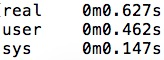
\includegraphics
	[width=0.3\textwidth]{image/time.jpg} 
	\caption{Sample output of the time command}.
\end{figure}
\begin{description}
	\item[$\cdot$] Real: This is the wall time mentioned above.
	\item[$\cdot$] User: User time is how much CPU time is spent in user mode.
	\item[$\cdot$] Sys: System time is how much CPU time is spent in kernel mode.
\end{description}
The difference between user- and kernel mode is the following:\\
In most memory protected systems there are some locked operations for security reasons. E.g. allocation of memory or accessing hardware requires kernel mode and cannot be done in user mode. Operations such as \textbf{malloc} and reading/writing to files will be processed by the kernel and are counted towards system time. This does not necessarily mean that all time is spent in kernel mode when for exampel reading a file, since the only time that is spent in kernel mode is reading the data from harddrive. The rest of the operation is counted towards user time. Therefore, to get the amount of time spent by the CPU, \textbf{User time} + \textbf{system time} is a good estimation. Another way to measure time spent on the CPU is to use the built in libraries. For example the \textbf{ThreadMXBean} in Java. This is especially useful for profiling.

\section{Materials and methods}
This section will address some details about the benchmarking and what material / software was used.
\subsection{Benchmarking}
Specs and language version: \\
Lenovo W530: Intel Core i5-3320M 2.60GHz x 4, 8GB RAM, Ubuntu 16.04 64-bit\\
MacBook (MacOne): Intel Core i5 1,4 GHz, 8 GB RAM, OS X El Capitan 10.11.5\\
MacBook (MacTwo): Intel Core i5 1,8 GHz, 4 GB RAM, OS X El Capitan 10.11.5\\
Julia 0.4.5 \\
Python 2.7.11+ \\
C++11 \\
Java 1.8.0\_92 \\\\
Benchmarking will be done by comparing the run time of the same algorithm in different languages. In this project the run time is measured as the sum of \textbf{system} and \textbf{user} time, because the \textbf{system} and \textbf{user} time are not affected by heavy loads on the machine. All time measurement are measured using the shell '\textbf{time}' command that returns the three types of time taken for the algorithm to run. The problems will be scaled to have smaller and larger inputs. However, in some situations a large input can cause memory problems, which will be addressed in the specific problem. The memory problems is unfortunately making an upper bound for how large data is possible to pass for certain problems. The time measurement is done by a software that was developed for this project. It runs test with different inputs a few times, calculates the median prints the result. 

\section{Problems}
In this section we explain some of the problems we have been using for benchmarking. One thing to keep in mind is that Java will do a lot of optimization and the reason to why we do not stop this, is because the optimization is a part of the Julia language, it is hard to get around and extra code is needed to trick Java not to do any optimizations. The goals is to benchmark the code of an average programmer the only rule is that every programming language has to do the same kind of operations, so it is important that Java does not stop beforehand because it checks to see that the result of what it is doing will never be used. A simple way to avoid this is to print the result or some parts of the result at the very end.
\subsection{Projecteuler 11}
\textit{In the 20$\times$20 grid below, four numbers along a diagonal line have been marked in red. The product of these numbers is 26$\times$63$\times$78$\times$14 = 1788696. What is the greatest product of four adjacent numbers in the same direction (up, down, left, right, or diagonally) in the 20$\times$20 grid?}
\begin{figure}[H]
	\begin{center}
	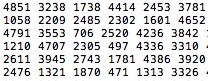
\includegraphics[scale=0.30]{image/11.jpg}
	\label{11}
	\end{center}
\end{figure}
The program runs from command-line/terminal with command line arguments in order to test on different inputs. To run the Julia version from the terminal: \\
\textbf{Julia euler11.jl 100 4}. \\
This would make the program run with a matrix of size 100 and calculating product of 4 adjacent numbers. A matrix generator was created to produce the matrix data,  which can be found in appendix. The matrix generator requires one argument, which is the size of the matrix. So if 500 is passed to the matrix generator, a file named \textbf{500mat.txt} will be created containing 500$\times$500 digits ranging from 100-9999.
\subsubsection{Solution}
The algorithm first reads through the input file and creates a matrix. To calculate products in all directions needed in the problem, the algorithm goes through the matrix a total of 3 times. A nested for loop is needed to go though a matrix, lines 1-2 at figure \ref{111}. The outer loop iterates through the rows, and the inner loop iterates through the columns. Figure \ref{111} calculates the horizontal and vertical directions, firgure \ref{112} diagonally from left to right(downwards) and figure \ref{113} going diagonally from right to left(downwards). The algorithm starts in the most upper left cell, and iterates through all cells in the matrix. Lets have the first cell as (1,1), first number is row(\textbf{i}) and second number is column(\textbf{j}). Looking at figure \ref{111}, \textbf{matLength} is the size of the matrix, size = 100 would mean a matrix of size $100 \cdot 100$. \textbf{numProd} is the number of adjacent numbers multiplied together. For matrix with size 100, and multiplying four adjacent numbers, the algorithm would do the following in figure \ref{111}: 
\begin{list}{}{}
	\item Starting at cell (1,1) to the end, which is cell (100, 100 - 4).
	\item Line 5-7: Loops over the adjacent cells and multiplies the numbers.
	\item Line 8-10: Sets current product to max product, if current is larger than previously max product.
\end{list}
\begin{figure}[H]
	\begin{center}
		\lstinputlisting[linerange={26-42}]{euler11.jl}
		\caption{Horizontal and vertical}
		\label{111}
	\end{center}
\end{figure}
Figure \ref{112} shows the loop that iterates over the matrix and calculating the product of the diagonal going downwards from left to right. Figure \ref{113} shows the diagonal product going upwards from left to right. The loop starts in the first row, and starting column is the last, not the first like the previously loops.
\begin{figure}[H]
	\begin{center}
		\lstinputlisting[linerange={47-55}]{euler11.jl}
		\caption{Diagonal downwards left to right}
		\label{112}
	\end{center}
\end{figure}
\begin{figure}[H]
	\begin{center}
		\lstinputlisting[linerange={60-68}]{euler11.jl}
		\caption{Diagonal upwards left to right}
		\label{113}
	\end{center}
\end{figure}
Figure \ref{graph112} and \ref{graph111} shows the test results of euler 11, keep in mind these results include the time for reading the input file and setting up the matrix. The test was made with 20 different inputs, matrices. Starting at 1000$\times$1000, increasing with 1000 in each test, and ending with 20.000$\times$20.000. Every test was with a product of 4 numbers. Figure \ref{graph113} shows how much time is used creating the matrix. Julia, Java and C++ uses most of the time reading the file and creating the matrix, and the actual work on the matrix is a small part of the total runtime. Python, on the other hand, uses most of the runtime working on the matrix. The test results of euler 11 shows that Java is the fastest, Julia is second, C++ third and Python fourth and last. Java is about 2-3 times faster than Julia and C++. Almost on all inputs Python is about ten times slower than Julia. In regards to “Graph making matrix” the time for Python uses to reading the file and creating the matrix is  This problem highlights one of the weaknesses of Python, arrays/lists. With Python being much slower than the rest of the languages, it was of course necessary to dig deeper to find out why. It turns out that arrays in Python are just really slow, and there is not much to do about it, unless external packages are included to help out. A package called \textbf{Numpy} should make operations on arrays much faster. The version in Python of euler 11 was tested with Python, and the results was worse than the regular version, and \textbf{Numpy} is not taken into account. Another thing to notice is that Julia is column-major when iterating over an matrix, where as the other languages are row-major. Column-major is that each column is loaded into memory, leading to iterating over a column is faster than iterating over a row. In this test Julia was implemented as iterating over rows before columns. For that reason a version of Julia was made that was column-major, figure \ref{graphopti} shows the comparison of regular version (row major), and the optimized version (column-major). This version also makes the matrix as column-major, meaning a row reading in the input file will become a column in the matrix. The mirroring of the matrix does not matter in this problem, as the product is calculated in all directions. On smaller inputs the runtime is lower, but not insignificantly lower. However, when the input increases in size, the difference between row-major and column-major becomes higher and higher. Looking at the six largest inputs, column-major is roughly 20\% faster than row-major, increasing the gap to Python.
\subsubsection{Results}
\begin{figure}[H]
	\centering
	\hspace*{-0.65in}
	\begin{subfigure}[b]{0.4\textwidth}
		\centering
		\scalebox{.8}{
		\begin{tikzpicture}
			\begin{axis} [
			title=Euler 11 - Julia,
			xlabel={$Input$},
			ylabel={$Time [s]$},
			grid=major,]
				\addplot [box plot median] table {graphdata/euler11-julia-box.dat};
				\addplot [box plot box] table {graphdata/euler11-julia-box.dat};
				\addplot [box plot top whisker] table {graphdata/euler11-julia-box.dat};
				\addplot [box plot bottom whisker] table {graphdata/euler11-julia-box.dat};
				\addplot table {graphdata/euler11-julia.dat};
			\end{axis}
		\end{tikzpicture}
		}
		\caption{}
		\label{boxplotjulia}
	\end{subfigure}
	\hfill
	\begin{subfigure}[b]{0.4\textwidth}
		\centering
		\scalebox{.8}{
		\begin{tikzpicture}
			\begin{axis} [
			title=Euler 11 - Python,
			xlabel={$Input$},
			ylabel={$Time [s]$},
			grid=major,]
				\addplot [box plot median] table {graphdata/euler11-python-box.dat};
				\addplot [box plot box] table {graphdata/euler11-python-box.dat};
				\addplot [box plot top whisker] table {graphdata/euler11-python-box.dat};
				\addplot [box plot bottom whisker] table {graphdata/euler11-python-box.dat};
				\addplot table {graphdata/euler11-python.dat};
			\end{axis}
		\end{tikzpicture}
		}
		\caption{}
		\label{boxplotpython}
	\end{subfigure}
	\hspace*{0.7in}
	\caption{}
\end{figure}
\begin{figure}[H]
	\centering
	\hspace*{-0.65in}
	\begin{subfigure}[H]{0.4\textwidth}
		\centering
		\scalebox{.8}{
		\begin{tikzpicture}
			\begin{axis} [
			title=Euler 11 - Java,
			xlabel={$Input$},
			ylabel={$Time [s]$},
			grid=major,]
				\addplot [box plot median] table {graphdata/euler11-java-box.dat};
				\addplot [box plot box] table {graphdata/euler11-java-box.dat};
				\addplot [box plot top whisker] table {graphdata/euler11-java-box.dat};
				\addplot [box plot bottom whisker] table {graphdata/euler11-java-box.dat};
				\addplot table {graphdata/euler11-java.dat};
			\end{axis}
		\end{tikzpicture}
		}
		\caption{}
		\label{boxplotjava}
	\end{subfigure}
	\hfill
	\begin{subfigure}[H]{0.4\textwidth}
		\centering
		\scalebox{.8}{
		\begin{tikzpicture}
			\begin{axis} [
			title=Euler 11 - C++,
			xlabel={$Input$},
			ylabel={$Time [s]$},
			grid=major,]
				\addplot [box plot median] table {graphdata/euler11-cpp-box.dat};
				\addplot [box plot box] table {graphdata/euler11-cpp-box.dat};
				\addplot [box plot top whisker] table {graphdata/euler11-cpp-box.dat};
				\addplot [box plot bottom whisker] table {graphdata/euler11-cpp-box.dat};
				\addplot table {graphdata/euler11-cpp.dat};
			\end{axis}
		\end{tikzpicture}
		}
		\caption{}
		\label{boxplotcpp}
	\end{subfigure}
	\hspace*{0.7in}
	\caption{}
\end{figure}
\begin{figure}[H]
	\centering
	\hspace*{-0.65in}
	\begin{subfigure}[H]{0.4\textwidth}
		\centering
		\scalebox{.8}{
		\begin{tikzpicture}
			\begin{axis} [
			title=Euler 11 - Julia optimized,
			xlabel={$Input$},
			ylabel={$Time [s]$},
			grid=major,]
				\addplot [box plot median] table {graphdata/euler11opti-julia-box.dat};
				\addplot [box plot box] table {graphdata/euler11opti-julia-box.dat};
				\addplot [box plot top whisker] table {graphdata/euler11opti-julia-box.dat};
				\addplot [box plot bottom whisker] table {graphdata/euler11opti-julia-box.dat};
				\addplot table {graphdata/euler11opti-julia.dat};
			\end{axis}
		\end{tikzpicture}
		}
		\caption{}
		\label{boxplotopti}
	\end{subfigure}
	\hfill
	\begin{subfigure}[H]{0.4\textwidth}
		\centering
		\scalebox{.8}{
		\begin{tikzpicture}
			\begin{axis}[
			title=Euler 11 - Julia comparison,
			xlabel={$Test Input$},
			ylabel={$Time [ms]$},
			grid=major,
			legend entries={$Julia$,$Julia\ optimized$},
			legend style={at={(1,1)},anchor=north west},
			]
			\addplot table {graphdata/euler11-julia.dat};
			\addplot table {graphdata/euler11opti-julia.dat};
			\end{axis}
		\end{tikzpicture}
		}
		\caption{}
		\label{graphopti}
	\end{subfigure}
	\hspace*{0.7in}
	\caption{}
\end{figure}
\begin{figure}[H]
	\centering
		\begin{tikzpicture}
			\begin{axis}[
			title=Euler 11 - Python excluded,
			xlabel={$Test Input$},
			ylabel={$Time [ms]$},
			grid=major,
			legend entries={$Julia$,$Java$,$c++$},
			legend style={at={(1,1)},anchor=north west},
			]
			\addplot table {graphdata/euler11-julia.dat};
			\addplot table {graphdata/euler11-java.dat};
			\addplot table {graphdata/euler11-cpp.dat};
			\end{axis}
		\end{tikzpicture}
	\caption{}
	\label{graph111}
\end{figure}
\begin{figure}[H]
	\centering
		\begin{tikzpicture}
			\begin{axis}[
			title=Euler 11,
			xlabel={$Test Input$},
			ylabel={$Time [ms]$},
			grid=major,
			legend entries={$Julia$,$Java$,$c++$,$Python$},
			legend style={at={(1,1)},anchor=north west},
			]
			\addplot table {graphdata/euler11-julia.dat};
			\addplot table {graphdata/euler11-java.dat};
			\addplot table {graphdata/euler11-cpp.dat};
			\addplot table {graphdata/euler11-python.dat};
			\end{axis}
		\end{tikzpicture}
	\caption{}
	\label{graph112}
\end{figure}
\begin{figure}[H]
	\centering
		\begin{tikzpicture}
			\begin{axis}[
			title=Euler 11 - File to matrix,
			xlabel={$Test Input$},
			ylabel={$Time [ms]$},
			grid=major,
			legend entries={$Julia$,$Java$,$c++$,$Python$},
			legend style={at={(1,1)},anchor=north west},
			]
			\addplot table {graphdata/euler11matmk-julia.dat};
			\addplot table {graphdata/euler11matmk-java.dat};
			\addplot table {graphdata/euler11matmk-cpp.dat};
			\addplot table {graphdata/euler11matmk-python.dat};
			\end{axis}
		\end{tikzpicture}
	\caption{}
	\label{graph113}
\end{figure}

\subsection{Projecteuler 116}
Description: \textit{A row of five black square tiles is to have a number of its tiles replaced with coloured oblong tiles from red(length two), green(length three), or blue(length four). If red tiles are chosen there are exactly seven ways. If green tiles are chosen there are three ways. And if blue tiles are chosen there are two ways. Figure \ref{116} is a visualization of how the tiles can be lain. Assuming that colours cannot be mixed there are $7+3+2=12$ ways of replacing the black tiles in a row measuring five units in length. How many different ways can the black tiles in a row measuring fifty units in length be replaced if colours cannot be mixed and at least one coloured tile must be used?}

\begin{figure}[H]
	\centering
	\begin{subfigure}[H]{0.6\textwidth}
		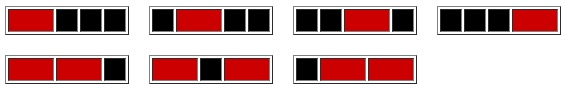
\includegraphics
		[width=\textwidth]{image/1161.jpg}
		\caption{Red tiles}.
	\end{subfigure}
	\begin{subfigure}[H]{0.6\textwidth}
		\centering
		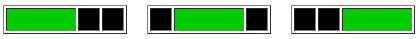
\includegraphics
		[width=\textwidth]{image/1162.jpg} 
		\caption{Green tiles}.
	\end{subfigure}	
	\begin{subfigure}[H]{0.6\textwidth}
		\centering
		
\includegraphics
		[width=\textwidth]{image/1163.jpg} 
		\caption{Blue tiles}.
	\end{subfigure}
	\caption{Projecteuler: 116}
	\label{116}
\end{figure}
\subsubsection{Solution}
The solution of this problem is done recursively, although an optimal solution would be done iterative. The work being done in every recursive call is very simple opposed to quicksort. When the work in every recursive call is simple and similar, some sort of compiler optimization will most likely happen if supported by the language. This is a good way to test Julia’s tail recursion optimization against Java's, and comparing with Python and C++.\\
\\
The above code is the solution written in Julia
\begin{lstlisting}
function solve(m::Int, n::Int) #m=color block size  n = black box size
  if m > n
    return 0
  end
  solutions = 0

  for i = m : n
    solutions += 1
    solutions += solve(m, n-i)
  end

  return solutions
end

function s(size::Int)
  result = 0;
  for i = 0 : 2
     result += solve(2+i, size)
  end
  return result
end

size = parse(Int, ARGS[1])
s(size)
\end{lstlisting}
The input that is changing when doing the benchmark is the size of the black box that's get filled with the three different sized blocks. The input will start at size 45 and increase by one every test. This will be done 10 times for each language. The result is a the following:
\subsubsection{Results}
It is clear that the graphs are exponential increasing. Another thing to notice is that the input is only increasing by one but is still making a huge difference in the run time. One of the reasons is that the problem is solved with recursion, for every extra one bit of space added to the black box a lot more recursive calls will have to be made.\\
\\
The difference in time between the four languages are as expected. Python does not support any form of tail recursion optimization and the result is really slow. Java and Julia on the other hand does a good job at optimizing the recursive calls and is actually faster than C++ - keep in mind that no compiler flags were used in C++, so the default optimization level is used.\\
\\
Julia and Java is close but Java is a bit faster, which is expected because of the fact that Java has been in development much longer than Julia and has a lot more optimization than Julia.

\begin{figure}[H]
	\centering
	\hspace*{-0.65in}
	\begin{subfigure}[b]{0.4\textwidth}
		\centering
		\scalebox{.8}{
		\begin{tikzpicture}
			\begin{axis} [
			title=Euler 116 - Julia,
			xlabel={$Input$},
			ylabel={$Time [s]$},
			grid=major,]
				\addplot [box plot median] table {graphdata/euler116ub-julia-box.dat};
				\addplot [box plot box] table {graphdata/euler116ub-julia-box.dat};
				\addplot [box plot top whisker] table {graphdata/euler116ub-julia-box.dat};
				\addplot [box plot bottom whisker] table {graphdata/euler116ub-julia-box.dat};
				\addplot table {graphdata/euler116ub-julia.dat};
			\end{axis}
		\end{tikzpicture}
		}
		\label{boxplot}
	\end{subfigure}
	\hfill
	\begin{subfigure}[b]{0.4\textwidth}
		\centering
		\scalebox{.8}{
		\begin{tikzpicture}
			\begin{axis} [
			title=Euler 116 - Python,
			xlabel={$Input$},
			ylabel={$Time [s]$},
			grid=major,]
				\addplot [box plot median] table {graphdata/euler116ub-python-box.dat};
				\addplot [box plot box] table {graphdata/euler116ub-python-box.dat};
				\addplot [box plot top whisker] table {graphdata/euler116ub-python-box.dat};
				\addplot [box plot bottom whisker] table {graphdata/euler116ub-python-box.dat};
				\addplot table {graphdata/euler116ub-python.dat};
			\end{axis}
		\end{tikzpicture}
		}
		\label{boxplot}
	\end{subfigure}
	\hspace*{0.7in}
\end{figure}
\begin{figure}[H]
	\centering
	\hspace*{-0.65in}
	\begin{subfigure}[H]{0.4\textwidth}
		\centering
		\scalebox{.8}{
		\begin{tikzpicture}
			\begin{axis} [
			title=Euler 116 - Java,
			xlabel={$Input$},
			ylabel={$Time [s]$},
			grid=major,]
				\addplot [box plot median] table {graphdata/euler116ub-java-box.dat};
				\addplot [box plot box] table {graphdata/euler116ub-java-box.dat};
				\addplot [box plot top whisker] table {graphdata/euler116ub-java-box.dat};
				\addplot [box plot bottom whisker] table {graphdata/euler116ub-java-box.dat};
				\addplot table {graphdata/euler116ub-java.dat};
			\end{axis}
		\end{tikzpicture}
		}
		\label{boxplot}
	\end{subfigure}
	\hfill
	\begin{subfigure}[H]{0.4\textwidth}
		\centering
		\scalebox{.8}{
		\begin{tikzpicture}
			\begin{axis} [
			title=Euler 116 - C++,
			xlabel={$Input$},
			ylabel={$Time [s]$},
			grid=major,]
				\addplot [box plot median] table {graphdata/euler116ub-cpp-box.dat};
				\addplot [box plot box] table {graphdata/euler116ub-cpp-box.dat};
				\addplot [box plot top whisker] table {graphdata/euler116ub-cpp-box.dat};
				\addplot [box plot bottom whisker] table {graphdata/euler116ub-cpp-box.dat};
				\addplot table {graphdata/euler116ub-cpp.dat};
			\end{axis}
		\end{tikzpicture}
		}
		\label{boxplot}
	\end{subfigure}
	\hspace*{0.7in}
\end{figure}
\begin{figure}[H]
	\centering
		\begin{tikzpicture}
			\begin{axis}[
			title=Euler 116 - Python excluded,
			xlabel={$Test Input$},
			ylabel={$Time [ms]$},
			grid=major,
			legend entries={$Julia$,$Java$,$c++$},
			legend style={at={(1,1)},anchor=north west},
			]
			\addplot table {graphdata/euler116ub-julia.dat};
			\addplot table {graphdata/euler116ub-java.dat};
			\addplot table {graphdata/euler116ub-cpp.dat};
			\end{axis}
		\end{tikzpicture}
	\caption{Graph}
	\label{graph}
\end{figure}
\begin{figure}[H]
	\centering
		\begin{tikzpicture}
			\begin{axis}[
			title=Euler 116,
			xlabel={$Test Input$},
			ylabel={$Time [ms]$},
			grid=major,
			legend entries={$Julia$,$Java$,$c++$,$Python$},
			legend style={at={(1,1)},anchor=north west},
			]
			\addplot table {graphdata/euler116ub-julia.dat};
			\addplot table {graphdata/euler116ub-java.dat};
			\addplot table {graphdata/euler116ub-cpp.dat};
			\addplot table {graphdata/euler116ub-python.dat};
			\end{axis}
		\end{tikzpicture}
	\caption{Graph}
	\label{graph}
\end{figure}

\subsection{Dual Piviot Quicksort}
Quicksort applies the divide-and-conquer paradigm to sort numbers. Dual pivot quicksort is very similar to the standard quicksort, the only difference is that instead of one pivot there are two pivots and three recursive calls. The first recursive call is the numbers that are less than the first pivot (which also must be the smallest of the two pivots). The second recursive call is with the numbers that are greater than the first pivot but less than the second pivot. The last recursive call is with the numbers greater than the second pivot. Dual pivot quicksort is so fast that it was not possible to get large enough data to get the run time close to 15 minutes. With a data set of 20.000.000 numbers the loading time was a few minutes while the sorting was only a few seconds. Much larger data set will cause out of memory error so it was necessary to change the approach. instead of sorting one big array, the program will first sort the elements from 0-125, then sort 0-250 and keep increasing the end index until the array size has been reached. This approach insures that the loading time of the data is so low that it does not matter in the full picture, but this way of doing quicksort cannot test how well quicksort performs with different inputs and is the reason why only uniform random inputs are used. \\
\\
The data set start at 100.000 numbers and increase by 30.000 every test. The solution is below:
\begin{lstlisting}
function quicksortDualPivot(a, s, e)
	if e > s

		if (a[s] > a[e])
	    	swap(a, s, e)
	    end

		leftPiv = a[s]
		rightPiv = a[e]

		leftPoi = s + 1
		rightPoi = e - 1

		curEle = leftPoi

		while curEle <= rightPoi
	    	if a[curEle] < leftPiv
	        	swap(a, curEle, leftPoi)
	        	leftPoi += 1
	    	elseif a[curEle] >= rightPiv
	        	while a[rightPoi] > rightPiv && curEle < rightPoi
	           		rightPoi -= 1
        		end

	        	swap(a, curEle, rightPoi)
	        	rightPoi -= 1
	        	if (a[curEle] < leftPiv)
	            	swap(a, curEle, leftPoi)
	            	leftPoi += 1
          		end
        	end
	        curEle += 1
        end
	    leftPoi -= 1
	    rightPoi += 1

	    swap(a, s, leftPoi)
	    swap(a, e, rightPoi)

	    quicksortDualPivot(a, s, leftPoi - 1)
	    quicksortDualPivot(a, leftPoi + 1, rightPoi - 1)
	    quicksortDualPivot(a, rightPoi + 1, e)
    end
end

function swap(a, i, j)
	tmp = a[i]
	a[i] = a[j]
	a[j] = tmp
end

#Load input
f = open(ARGS[1])
s = readall(f)
ss = split(s)
data = []
for i = 1 : length(ss)
	push!(data, parse(Int32, ss[i]))
end
close(f)


jumpLength = 125
i = 0
shouldBreak = false;

while true
	i += jumpLength
	if i > length(data)
		i = length(data)
		shouldBreak = true
	end

	quicksortDualPivot(data, 1, i)

	if shouldBreak == true
		break
	end
end
\end{lstlisting}
\subsubsection{Results}
The fastest of the four languages is definitely Java, which is kind of surprising as the expectation was that the compiler optimization would break with this kind of work in every recursive call - to check if Java was over optimizing a few elements from the sorted list was printed at the end of the program, to insure Java did not just terminate because it found that the array was not going to be used further after the sorting. Although Javas optimization is still present, the optimization of Julia's breaks and has a hard time to complete the first few inputs. C++ seems pretty slow compared to Java but keep in mind that this is without much optimization - C++ is known for the fast speed performance when working with arrays and this is why it does manage to get almost all inputs opposed to Python, which has no recursion optimization and is really slow when working with arrays and lists.

\begin{figure}[H]
	\centering
	\hspace*{-0.65in}
	\begin{subfigure}[b]{0.4\textwidth}
		\centering
		\scalebox{.8}{
		\begin{tikzpicture}
			\begin{axis} [
			title=Quicksort - Julia,
			xlabel={$Input$},
			ylabel={$Time [s]$},
			grid=major,]
				\addplot [box plot median] table {graphdata/quicksort-julia-box.dat};
				\addplot [box plot box] table {graphdata/quicksort-julia-box.dat};
				\addplot [box plot top whisker] table {graphdata/quicksort-julia-box.dat};
				\addplot [box plot bottom whisker] table {graphdata/quicksort-julia-box.dat};
				\addplot table {graphdata/quicksort-julia.dat};
			\end{axis}
		\end{tikzpicture}
		}
		\label{boxplot}
	\end{subfigure}
	\hfill
	\begin{subfigure}[b]{0.4\textwidth}
		\centering
		\scalebox{.8}{
		\begin{tikzpicture}
			\begin{axis} [
			title=Quicksort - Python,
			xlabel={$Input$},
			ylabel={$Time [s]$},
			grid=major,]
				\addplot [box plot median] table {graphdata/quicksort-python-box.dat};
				\addplot [box plot box] table {graphdata/quicksort-python-box.dat};
				\addplot [box plot top whisker] table {graphdata/quicksort-python-box.dat};
				\addplot [box plot bottom whisker] table {graphdata/quicksort-python-box.dat};
				\addplot table {graphdata/quicksort-python.dat};
			\end{axis}
		\end{tikzpicture}
		}
		\label{boxplot}
	\end{subfigure}
	\hspace*{0.7in}
\end{figure}
\begin{figure}[H]
	\centering
	\hspace*{-0.65in}
	\begin{subfigure}[H]{0.4\textwidth}
		\centering
		\scalebox{.8}{
		\begin{tikzpicture}
			\begin{axis} [
			title=Quicksort - Java,
			xlabel={$Input$},
			ylabel={$Time [s]$},
			grid=major,]
				\addplot [box plot median] table {graphdata/quicksort-java-box.dat};
				\addplot [box plot box] table {graphdata/quicksort-java-box.dat};
				\addplot [box plot top whisker] table {graphdata/quicksort-java-box.dat};
				\addplot [box plot bottom whisker] table {graphdata/quicksort-java-box.dat};
				\addplot table {graphdata/quicksort-java.dat};
			\end{axis}
		\end{tikzpicture}
		}
		\label{boxplot}
	\end{subfigure}
	\hfill
	\begin{subfigure}[H]{0.4\textwidth}
		\centering
		\scalebox{.8}{
		\begin{tikzpicture}
			\begin{axis} [
			title=Quicksort - C++,
			xlabel={$Input$},
			ylabel={$Time [s]$},
			grid=major,]
				\addplot [box plot median] table {graphdata/quicksort-cpp-box.dat};
				\addplot [box plot box] table {graphdata/quicksort-cpp-box.dat};
				\addplot [box plot top whisker] table {graphdata/quicksort-cpp-box.dat};
				\addplot [box plot bottom whisker] table {graphdata/quicksort-cpp-box.dat};
				\addplot table {graphdata/quicksort-cpp.dat};
			\end{axis}
		\end{tikzpicture}
		}
		\label{boxplot}
	\end{subfigure}
	\hspace*{0.7in}
\end{figure}
\begin{figure}[H]
	\centering
		\begin{tikzpicture}
			\begin{axis}[
			title=Quicksort,
			xlabel={$Test Input$},
			ylabel={$Time [ms]$},
			grid=major,
			legend entries={$Julia$,$Java$,$c++$,$Python$},
			legend style={at={(1,1)},anchor=north west},
			]
			\addplot table {graphdata/quicksort-julia.dat};
			\addplot table {graphdata/quicksort-java.dat};
			\addplot table {graphdata/quicksort-cpp.dat};
			\addplot table {graphdata/quicksort-python.dat};
			\end{axis}
		\end{tikzpicture}
	\caption{Graph}
	\label{graph}
\end{figure}

\subsection{Statistics}
To obtain a broader perspective on the behavior of the languages, in addition to the three problems analyzed in the previous chapters we have also performed a comprehensive testing on a set of problems from Project Euler.
In the statistics there are 15 problems from Project Euler, which corresponds to 60 separate programs. The running times of solutions to the Project Euler problems, as originally stated, mostly take less than a second. Since the differences of the order of milliseconds are not that significant and such benchmarks might be susceptible to measurement of errors, we have scaled the problems. Every given problem was tested with ten different inputs. The first input is as stated in the original problem, and then increased nine times, giving ten results for each problem. There was set a maximum run time of five minutes for each test. All programs were tested three times with each input, and the median is used for the graphs shown below. 
Starting with 60 programs, each is tested with ten different inputs and each input is tested three times, resulting in 1800 program runs. Keeping the amount of programs in mind, an average run time of one minute, would make the testing phase to a total of 30 hours for one computer. 
Therefore, the testing was divided to run on three computers. The specifications of the computers can be seen in section \textbf{6.1 Benchmarking}. MacOne tested eulers: 1, 4, 8, 9, 12 and 13. Lenovo tested eulers: 14, 16 and 21. MacTwo tested eulers: 30, 31, 36, 50, 52, 76 and 112.
One problem which we have encountered and which turned out to be time consuming is that the inputs had only been properly tested on the Julia versions, before making the final tests. In some cases, the other languages, opposed to Julia, had trouble going through all inputs within the time limit. All programs were implemented in Julia as the first language, and implemented in Python, Java and C++. A consequence is that the problems are not optimized in a certain language, possibly giving Julia an advantage over the other languages. This advantage might be true, since Julia is the only language to finish all the programs with all inputs.
If a test exceeds the time limit of five minutes, it will not be included in the graphs shown.
Some of the problems had to be altered in order to being able to handle large inputs. Problem 8 and 13 all reads their inputs from a .txt file, before doing any computations. The time for reading data from a file and setting up the data, is 
included in the run time of the tests.

\begin{figure}[H]
	\centering
	\hspace*{-0.65in}
	\begin{subfigure}[b]{0.4\textwidth}
		\centering
		\scalebox{.8}{
		\begin{tikzpicture}
			\begin{axis} [
			title=Euler 1,
			xlabel={$Input$},
			ylabel={$Time [s]$},
			grid=major,]
			\addplot table {graphdata/euler1-julia.dat};
			\addplot table {graphdata/euler1-java.dat};
			\addplot table {graphdata/euler1-cpp.dat};
			\addplot table {graphdata/euler1-python.dat};
			\end{axis}
		\end{tikzpicture}
		}
		\label{boxplot}
	\end{subfigure}
	\hfill
	\begin{subfigure}[b]{0.4\textwidth}
		\centering
		\scalebox{.8}{
		\begin{tikzpicture}
			\begin{axis} [
			title=Euler 4,
			xlabel={$Input$},
			ylabel={$Time [s]$},
			grid=major,
			legend entries={$Julia$,$Java$,$c++$,$Python$},
			legend style={at={(1,1)},anchor=north west},
			]
			\addplot table {graphdata/euler4-julia.dat};
			\addplot table {graphdata/euler4-java.dat};
			\addplot table {graphdata/euler4-cpp.dat};
			\addplot table {graphdata/euler4-python.dat};
			\end{axis}
		\end{tikzpicture}
		}
		\label{boxplot}
	\end{subfigure}
	\hspace*{0.7in}
\end{figure}
\begin{figure}[H]
	\centering
	\hspace*{-0.65in}
	\begin{subfigure}[b]{0.4\textwidth}
		\centering
		\scalebox{.8}{
		\begin{tikzpicture}
			\begin{axis} [
			title=Euler 8,
			xlabel={$Input$},
			ylabel={$Time [s]$},
			grid=major,]
			\addplot table {graphdata/euler8-julia.dat};
			\addplot table {graphdata/euler8-java.dat};
			\addplot table {graphdata/euler8-cpp.dat};
			\end{axis}
		\end{tikzpicture}
		}
		\label{boxplot}
	\end{subfigure}
	\hfill
	\begin{subfigure}[b]{0.4\textwidth}
		\centering
		\scalebox{.8}{
		\begin{tikzpicture}
			\begin{axis} [
			title=Euler 9,
			xlabel={$Input$},
			ylabel={$Time [s]$},
			grid=major,
			legend entries={$Julia$,$Java$,$c++$,$Python$},
			legend style={at={(1,1)},anchor=north west},
			]
			\addplot table {graphdata/euler9-julia.dat};
			\addplot table {graphdata/euler9-java.dat};
			\addplot table {graphdata/euler9-cpp.dat};
			\addplot table {graphdata/euler9-python.dat};
			\end{axis}
		\end{tikzpicture}
		}
		\label{boxplot}
	\end{subfigure}
	\hspace*{0.7in}
\end{figure}
\begin{figure}[H]
	\centering
	\hspace*{-0.65in}
	\begin{subfigure}[b]{0.4\textwidth}
		\centering
		\scalebox{.8}{
		\begin{tikzpicture}
			\begin{axis} [
			title=Euler 13,
			xlabel={$Input$},
			ylabel={$Time [s]$},
			grid=major,]
			\addplot table {graphdata/euler13-julia.dat};
			\addplot table {graphdata/euler13-java.dat};
			\addplot table {graphdata/euler13-cpp.dat};
			\addplot table {graphdata/euler13-python.dat};
			\end{axis}
		\end{tikzpicture}
		}
		\label{boxplot}
	\end{subfigure}
	\hfill
	\begin{subfigure}[b]{0.4\textwidth}
		\centering
		\scalebox{.8}{
		\begin{tikzpicture}
			\begin{axis} [
			title=Euler 14,
			xlabel={$Input$},
			ylabel={$Time [s]$},
			grid=major,
			legend entries={$Julia$,$Java$,$c++$,$Python$},
			legend style={at={(1,1)},anchor=north west},
			]
			\addplot table {graphdata/euler14-julia.dat};
			\addplot table {graphdata/euler14-java.dat};
			\addplot table {graphdata/euler14-cpp.dat};
			\addplot table {graphdata/euler14-python.dat};
			\end{axis}
		\end{tikzpicture}
		}
		\label{boxplot}
	\end{subfigure}
	\hspace*{0.7in}
\end{figure}
\begin{figure}[H]
	\centering
	\hspace*{-0.65in}
	\begin{subfigure}[b]{0.4\textwidth}
		\centering
		\scalebox{.8}{
		\begin{tikzpicture}
			\begin{axis} [
			title=Euler 16,
			xlabel={$Input$},
			ylabel={$Time [s]$},
			grid=major,]
			\addplot table {graphdata/euler16-julia.dat};
			\addplot table {graphdata/euler16-java.dat};
			\addplot table {graphdata/euler16-cpp.dat};
			\addplot table {graphdata/euler16-python.dat};
			\end{axis}
		\end{tikzpicture}
		}
		\label{boxplot}
	\end{subfigure}
	\hfill
	\begin{subfigure}[b]{0.4\textwidth}
		\centering
		\scalebox{.8}{
		\begin{tikzpicture}
			\begin{axis} [
			title=Euler 21,
			xlabel={$Input$},
			ylabel={$Time [s]$},
			grid=major,
			legend entries={$Julia$,$Java$,$c++$,$Python$},
			legend style={at={(1,1)},anchor=north west},
			]
			\addplot table {graphdata/euler21-julia.dat};
			\addplot table {graphdata/euler21-java.dat};
			\addplot table {graphdata/euler21-cpp.dat};
			\addplot table {graphdata/euler21-python.dat};
			\end{axis}
		\end{tikzpicture}
		}
		\label{boxplot}
	\end{subfigure}
	\hspace*{0.7in}
\end{figure}
\begin{figure}[H]
	\centering
	\hspace*{-0.65in}
	\begin{subfigure}[b]{0.4\textwidth}
		\centering
		\scalebox{.8}{
		\begin{tikzpicture}
			\begin{axis} [
			title=Euler 30,
			xlabel={$Input$},
			ylabel={$Time [s]$},
			grid=major,]
			\addplot table {graphdata/euler30-julia.dat};
			\addplot table {graphdata/euler30-java.dat};
			\addplot table {graphdata/euler30-cpp.dat};
			\addplot table {graphdata/euler30-python.dat};
			\end{axis}
		\end{tikzpicture}
		}
		\label{boxplot}
	\end{subfigure}
	\hfill
	\begin{subfigure}[b]{0.4\textwidth}
		\centering
		\scalebox{.8}{
		\begin{tikzpicture}
			\begin{axis} [
			title=Euler 31,
			xlabel={$Input$},
			ylabel={$Time [s]$},
			grid=major,
			legend entries={$Julia$,$Java$,$c++$,$Python$},
			legend style={at={(1,1)},anchor=north west},
			]
			\addplot table {graphdata/euler31-julia.dat};
			\addplot table {graphdata/euler31-java.dat};
			\addplot table {graphdata/euler31-cpp.dat};
			\addplot table {graphdata/euler31-python.dat};
			\end{axis}
		\end{tikzpicture}
		}
		\label{boxplot}
	\end{subfigure}
	\hspace*{0.7in}
\end{figure}

\begin{figure}[H]
	\centering
	\hspace*{-0.35in}
	\begin{subfigure}[b]{0.4\textwidth}
		\centering
		\scalebox{.8}{
		\begin{tikzpicture}
			\begin{axis} [enlarge x limits=0.5, xtick = data, ylabel={$Time [s]$},]
				\addplot [box plot median] table {graphdata/stats-julia.dat};
				\addplot [box plot box] table {graphdata/stats-julia.dat};
				\addplot [box plot top whisker] table {graphdata/stats-julia.dat};
				\addplot [box plot bottom whisker] table {graphdata/stats-julia.dat};
			\end{axis}
		\end{tikzpicture}
		}
		\caption{Stats: Julia}
		\label{boxplot}
	\end{subfigure}
	\hfill
	\begin{subfigure}[b]{0.4\textwidth}
		\centering
		\scalebox{.8}{
		\begin{tikzpicture}
			\begin{axis} [enlarge x limits=0.5, xtick = data, ylabel={$Time [s]$},]
				\addplot [box plot median] table {graphdata/stats-python.dat};
				\addplot [box plot box] table {graphdata/stats-python.dat};
				\addplot [box plot top whisker] table {graphdata/stats-python.dat};
				\addplot [box plot bottom whisker] table {graphdata/stats-python.dat};
			\end{axis}
		\end{tikzpicture}
		}
		\caption{Stats: Python}
		\label{boxplot}
	\end{subfigure}
	\hspace*{0.53in}
\end{figure}
\begin{figure}[H]
	\centering
	\hspace*{-0.35in}
	\begin{subfigure}[b]{0.4\textwidth}
		\centering
		\scalebox{.8}{
		\begin{tikzpicture}
			\begin{axis} [enlarge x limits=0.5, xtick = data, ylabel={$Time [s]$},]
				\addplot [box plot median] table {graphdata/stats-java.dat};
				\addplot [box plot box] table {graphdata/stats-java.dat};
				\addplot [box plot top whisker] table {graphdata/stats-java.dat};
				\addplot [box plot bottom whisker] table {graphdata/stats-java.dat};
			\end{axis}
		\end{tikzpicture}
		}
		\caption{Stats: Java}
		\label{boxplot}
	\end{subfigure}
	\hfill
	\begin{subfigure}[b]{0.4\textwidth}
		\centering
		\scalebox{.8}{
		\begin{tikzpicture}
			\begin{axis} [enlarge x limits=0.5, xtick = data, ylabel={$Time [s]$},]
				\addplot [box plot median] table {graphdata/stats-cpp.dat};
				\addplot [box plot box] table {graphdata/stats-cpp.dat};
				\addplot [box plot top whisker] table {graphdata/stats-cpp.dat};
				\addplot [box plot bottom whisker] table {graphdata/stats-cpp.dat};
			\end{axis}
		\end{tikzpicture}
		}
		\caption{Stats: C++}
		\label{boxplot}
	\end{subfigure}
	\hspace*{0.53in}
\end{figure}
\begin{figure}[H]
	\centering
	\begin{tikzpicture}
		\begin{axis} [enlarge x limits=0.5, xtick = data, ylabel={$Time [s]$},]
			\addplot [box plot median] table {graphdata/stats-julia.dat};
			\addplot [box plot median] table {graphdata/stats-python.dat};
			\addplot [box plot median] table {graphdata/stats-java.dat};
			\addplot [box plot median] table {graphdata/stats-cpp.dat};
			\addplot [box plot box] table {graphdata/stats-julia.dat};
			\addplot [box plot box] table {graphdata/stats-python.dat};
			\addplot [box plot box] table {graphdata/stats-java.dat};
			\addplot [box plot box] table {graphdata/stats-cpp.dat};
		\end{axis}
	\end{tikzpicture}
	\caption{Stats without whiskers: 1 Julia, 2 Python, 3 Java and 4 C++}
	\label{boxplot}
\end{figure}
\begin{figure}[H]
	\centering
	\begin{tikzpicture}
		\begin{axis} [enlarge x limits=0.5, xtick = data, ylabel={$Time [s]$},]
			\addplot [box plot median] table {graphdata/stats-julia.dat};
			\addplot [box plot median] table {graphdata/stats-python.dat};
			\addplot [box plot median] table {graphdata/stats-java.dat};
			\addplot [box plot median] table {graphdata/stats-cpp.dat};
			\addplot [box plot box] table {graphdata/stats-julia.dat};
			\addplot [box plot box] table {graphdata/stats-python.dat};
			\addplot [box plot box] table {graphdata/stats-java.dat};
			\addplot [box plot box] table {graphdata/stats-cpp.dat};
			\addplot [box plot top whisker] table {graphdata/stats-julia.dat};
			\addplot [box plot top whisker] table {graphdata/stats-python.dat};
			\addplot [box plot top whisker] table {graphdata/stats-java.dat};
			\addplot [box plot top whisker] table {graphdata/stats-cpp.dat};
			\addplot [box plot bottom whisker] table {graphdata/stats-julia.dat};
			\addplot [box plot bottom whisker] table {graphdata/stats-python.dat};
			\addplot [box plot bottom whisker] table {graphdata/stats-java.dat};
			\addplot [box plot bottom whisker] table {graphdata/stats-cpp.dat};
		\end{axis}
	\end{tikzpicture}
	\caption{Stats with whiskers: 1 Julia, 2 Python, 3 Java and 4 C++}
	\label{boxplot}
\end{figure}

\section{Personal experience with Julia}
In this section we each wrote about our personal experience with Julia.
\subsection{Sonni}
Some of the design choices in Julia can be really frustrating for someone who is adapting to Julia. The indices starts at 1 - this could be debatable because of the statement that Julia is used in a lot of scientific computations and many programming languages made for scientific computations use 1-based indexing. But as a programmer who is used to indices starting at 0, this can cause a lot of unnecessary bugs. The developers of Julia also made unusual design choice with the for-loop syntax. A incrementing for loop looks like:
\begin{lstlisting}[language=python]
Julia:
for i = 1 : n
	Some code ...
end

General languages:
for i = 1; i < n; i++
	Some code ...
\end{lstlisting}
This is straightforward in many other languages, but take a look at the decrementing for-loop:
\begin{lstlisting}[language=python]
Julia:
for i = n : -1 : 0
	Some code ...
end

General languages:
for i = n; i > 0; i--
	Some code
\end{lstlisting}
In Julia the exit condition and incrementation / decrementation are swapped and there is no consistency. The decrementing for-loops both start at textbf{n}, and stops at 0. This kind of syntax can again cause bugs, and is not that easy to get used to.\\
\\
The documentation of Julia is far from being great, which is a huge bump on the road to learn Julia. It feels far from complete. The documentation does not explain much but instead gives some examples. Essential information are often lacking, e.g. what types are needed by a given function. It might point out that these arguments are needed, but do not describe those arguments. An example from the documentation is the function \textbf{rand()}, which is used to generate random numbers:

\begin{lstlisting}
rand( [ rng ] [ ,S ] [ , dims... ] )
\end{lstlisting} 
\say{Pick a random element or array of random elements from the set of values specified by S; S can be:\\
- an indexable collection (for example 1:n or ['x','y','z']), or  \\
- a type: the set of values to pick from is then equivalent to typemin(S):typemax(S) for integers (this is not applicable to BigInt), and to [0,1) for floating point numbers;  \\
S defaults to Float64.} \\
The argument \textbf{S} is explained, but the documentations does not mention anything about \textbf{rng} or \textbf{dims}.\\
Another example is how to access data within an array at a specific index. This should be one of the first things in the Array section, but is first described after about two pages of text. A person with experience in programming might know that to access an element in an array with an index is this simple line of code:
\begin{lstlisting}
a[index]
\end{lstlisting} 
But this isn’t so obvious for new programmers. It is clear that something has to be done with the documentation.\\
\\ 
Another downside to Julia is its consistency. The developers has tried to remove some of the burden from the programmer with dynamic typing, package manager system etc., but with memory allocation and garbage collection it does not make much sense. The garbage collector does not free memory from unreachable object. Sizes of variables cannot be changed after declaration, and is not automatically increased if needed. If the programmer assign for example 8 bit memory to a variable and later change the value of that variable, then julia automatically assigns 32 bit or more if needed to that variable even if the 8 bits were enough. 
\subsection{Simon}
I personally see myself as the one in the group with the least programming experience, and might needed more time learning Julia. I was not learning as fast as the others. I only know a few languages, and as many know, the more languages you know, the easier it gets learning a new language. The documentation of Julia was not satisfying enough to me. I learn faster if I can visually see how a function is used, rather than reading a wall of text. The visualizations of the current documentation were not fulfilling my needs. The documentation also misses to explain crucial information to a function, like what a given argument is presenting. For that reason I often found myself looking through the documentation of Python, to read about a function, since the syntax is so similar. Nevertheless, for programming I keep finding Julia more satisfying as I learn more, and for future programming I will definitely use Julia over Python.

\subsection{Asbjørn}
I found the syntax a bit confusing at first. I am not used to Python and I missed code structure and forced typing, in Julia and Python it looks like the code is hovering. After some time I got used to it and I found it very easy to learn. It makes it a little hard to find answers with the documentation and community being a bit smaller than with other languages. I think the 1-indexing is a bit complicated because I had never thought any language would use this, but I found that a lot of languages actually use this, they just are not that popular.

\section{Discussion}
From personal experience we found that Julia is easy to learn even for beginners. For a programmer who is familiar with Python should not have a hard time getting used to Julia. The easy to learn syntax might have had a cost. Again, from our personal experience some of us find the syntax less readable than programming languages with parenthesis/bracket structure. A lot of people seem excited about the new language. 
In out tests Julia is much faster than Python, but does this mean Julia is better? In out test it would be yes, but the fact that Julia is still young and Python have a lot of useful libraries developed over the years makes Python a little more useful. A programmer who got a lot of experience in Python knows how to make it almost as fast as C. Julia is better at being simple and nobody knows what the developers can accomplish before Julia hit full version.
Why should a programmer choose julia for his project? One of the reasons to use Julia is the wide range of features and the fact that it should take long to develop a prototype. The reason not to is mostly personal reasons or the fact that their documentation is very poor. Julia is so far a useful language, but it needs the same community and trust as many of the larger languages to break through.
 

\section{Conclusion}
It can be difficult to make any conclusions by the benchmarking but it may give an idea of how Julia performs, compared to Java, Python and C++. One thing to keep in mind is that as of writing this report, Julia is in version 0.4.5 - it has yet to reach version 1.0.0 while the other languages are much older than Julia. This could mean that Julia might get even faster in the future and by the benchmarking it does look like that Julia is already performing well. The idea of the developers is clear, they are trying to make a programming language that is as easy to learn and write as Python but with a compiler that optimizes code like Java and both of these goals have more or less been reached by the developers. Julia was definitely easy to learn and by the benchmarking it does look like that the compiler is doing well with the optimization when it is possible. It does also feels like that the Julia developers are playing with the idea of giving the user some control over what is happening behind the scene. ‘Playing’ because this does not feel close to done. There are examples where they are giving the user an option to allocate memory for variables manually, but as soon as a new value is assign to that variable then Julia will change the memory size. Also it is not possible to free a declared variables memory entirely and the only operation the user can do with the garbage collector is force garbage collection and disable the garbage collector. Similarly, it seems that the option to implement code from other languages this seems kind of buggy and not complete.

\newpage
\section{Appendix}
\subsection{Process analysis}
This section is about our management of time and resources.
\subsubsection{Projectmanagement, organizing workflow and organizing process of learning}
The first thing we agreed doing was getting to know Julia for the research. We used a lot of time solving problems in Julia and trying to figure out how to get a view of what was to be done and how to organize it. We mostly communicated through facebook and created a repository on github to share project files. We gathered our solutions to Project Euler and made comparisons. Gathering information about benchmarking we mostly ran into walls of text on how to do it properly, and did not know where to start. Every time we thought we were understanding benchmarking, our supervisor taught us something new. We created a board on Trello. We made a to-do list of cards so we knew what had to be done and started handing out tasks. We communicated more with our supervisor via email as we started writing the report. The group was really good at getting the tasks, we agreed on doing, done. We should have been using more tools for organizing and we did not set any deadlines for anything. Scrum is a tool, which would have helped us a lot, but it is not that easy to learn. We should have met and worked together, several times a week, discussing our problems and goals. 

\subsubsection{Process of learning}
We learned by both direct and indirect learning process. We learned Julia indirectly by solving Project Euler. We pretty much read about every topic, which is direct learning. We cannot think of another way to learn programming than reading, trying it out and reading to get a result. Project Euler was a good support for learning, since learning something new, is much easier, when there's a purpose or a goal. Programming is not as fun if there's no end goal in mind.

\subsubsection{Cooperation, difficulties in group and with supervisor}
We actually had a good idea about who was good at what and splitting the tasks between us with this in mind. The communication could have been better. It seemed that we worked on different times of the day, which made communication difficult. Our supervisor did his best and we think he did a good job.

\subsubsection{Conclusion}
Trello is a very good tool for organizing and we should have been using it from the beginning. Looking beyond the fact that some data was lost using Git, the tool is perfect for team programming. We have payed the price not making any deadlines. Deadlines seems useless when the focus is just on the project, but when the workload gets more intense, it can be very good to have smaller deadlines or milestones during a project. Meetings should have occured more often, and syncing the current progress. Overall collaboration was very well, taken into account what could have been improved.

\begin{thebibliography}{9}
	
	\bibitem{cormen}
	Thomas H. Cormen, Charles E. Leiserson, Ronald Rivest, Clifford Stein
	\emph{Introduction to Algorithms},
	Cambridge, Massachusetts,
	third edition,
	2009.
	\bibitem{toplst}
	\url{http://www.tiobe.com/tiobe\_index}
	\bibitem{ju-why}
	\url{http://julialang.org}
	\bibitem{ju-uni}
	\url{http://unicode.org/standard/WhatIsUnicode.html}
	\bibitem{ju-vec}
	\url{http://www.cs.cornell.edu/courses/cs1112/2013fa/Exams/exam2/vectorizedCode.pdf}
	\bibitem{ju-py}
	\url{https://www.ibm.com/developerworks/community/blogs/jfp/entry/Python_Meets_Julia_Micro_Performance?lang=en}
	\bibitem{li-thr}
	\url{https://www.techopedia.com/definition/24784/lightweight-thread}
	\bibitem{user-sys}
	\url{http://stackoverflow.com/questions/556405/what-do-real-user-and-sys-mean-in-the-output-of-time1}
	\url{http://www.evanmiller.org/why-im-betting-on-julia.html}
	\url{http://julialang.org/}
	\url{http://www.nowozin.net/sebastian/blog/the-julia-language-for-scientific-computing.html}
	\url{http://radar.oreilly.com/2013/10/julias-role-in-data-science.html}
\end{thebibliography}

\end{document}

